\documentclass[a4paper,12pt]{article}
\usepackage{amsmath}  % Pour les symboles mathématiques
\usepackage{amssymb}  % Pour les ensembles comme Z
\usepackage{graphicx}  % Pour inclure des images
\usepackage{geometry}  % Pour les marges
\usepackage{fancyhdr}  % Pour les en-têtes et pieds de page
\usepackage{tkz-tab} % Pour les tableau de variation

\geometry{top=3cm, bottom=3cm, left=2.5cm, right=2.5cm}
\pagestyle{fancy}
\fancyhf{}
\fancyhead[L]{Correction TD Généralité 2, Groupe 1}
\fancyhead[R]{}
\fancyfoot[C]{\thepage}
\setcounter{secnumdepth}{0}

\title{\textbf{Correction TD Généralité 2 : Ensemble (Groupe 1)}}
\author{Ethan VERMOT DESROCHES}
\date{26 Septembre 2024}

\begin{document}

\maketitle
\thispagestyle{fancy}
\section*{Disclaimer}
Cette correction est loin d'être parfaite. Des erreurs ou imprécisions peuvent s'y glisser. Si vous trouvez des erreurs / faute d’orthographe / imprécision (ce qui est très probable), alors dite le moi (@knahte sur Discord).
\tableofcontents
\newpage

\section{Exercice 1}
\subsection{Exercice 1.1}
Déterminer l'ensemble :
\[
\left\{ x + \frac{1}{x} \mid x \in \mathbb{R}^{+*} \right\}
\]
Soit l'ensemble $E$
\[
E = \left\{ x + \frac{1}{x} \mid x \in \mathbb{R}^{+*} \right\}
\]
Soit la fonction $f$ définie par :
\[
\begin{aligned}
f :& \mathbb{R}^{+*} \to \mathbb{R}^{+*}
\\
& x \mapsto x + \frac{1}{x}
\end{aligned}
\]
$f$ est dérivable sur $\mathbb{R}^{+*}$
\[
\forall x \in \mathbb{R}^{+*}, \quad f'(x) = 1 - \frac{1}{x^2}
\]

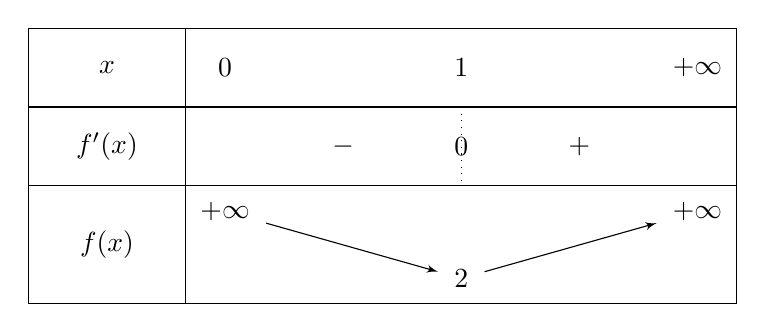
\begin{tikzpicture}
   \tkzTabInit{$x$ / 1 , $f'(x)$ / 1, $f(x)$ / 1.5}{$0$, $1$, $+\infty$}
   \tkzTabLine{, -, z, +, }
   \tkzTabVar{+/ $+\infty$, -/ $2$, +/ $+\infty$}
\end{tikzpicture}
\\
2 est donc le minimum de $f$:
\[
\forall x \in \mathbb{R}^{+*}, \quad f'(x) \in [ 2; +\infty[
\]
Ainsi, par le théorème des valeurs intermédiaire,
\[
\forall y \in[ 2; +\infty[ = [ f(1); \lim_{+\infty} f [ ,\quad \exists x \in [ 1; +\infty[, f(y) = x
\]
Ainsi
\[
[ 2 ; + \infty [ \subset E
\]
\textbf{Par double inclusion, $E = [ 2 ; + \infty [$}


\subsection{Exercice 1.2}
Déterminer l'ensemble :
\[
 \left\{ y \in \mathbb{R}, \exists x \in \mathbb{R}, x^2 + 2xy + y^4 = 0 \right\}
\]
Soit l'ensemble $F$
\[
F = \left\{ y \in \mathbb{R}, \exists x \in \mathbb{R}, x^2 + 2xy + y^4 = 0 \right\}
\]
Soit $y \in \mathbb{R}^{+*}$
On résout l'équation du 2nd degré d’inconnu $x \in \mathbb{R}$
\[
x^2 + 2xy + y^4 = 0
\]
\[
\begin{aligned}
\Delta &= (2y^2) - 4y^4\\
&= 4y^2 (1 - y^2)
\end{aligned}
\]
L'équation du 2nd degré admet des solutions réelles si et seulement si 
\[
\Delta > 0
\]
Or
\[
4y^2 > 0
\]
Donc 
\[
\begin{aligned}
\Delta \ge 0  \Leftrightarrow & (1-y^2) \ge 0\\
\Leftrightarrow& y^2 \le 1\\
\Leftrightarrow& -1 \le y \le 1
\end{aligned}
\]
Ainsi
\[
-1 \le y \le 1 \Leftrightarrow \exists x \in \mathbb{R}, x^2 + 2xy + y^4 = 0
\]
\textbf{Donc $F = [-1 ; 1]$}
\section{Exercice 2}
\subsection{Exercice 2.1}
\subsubsection{Exercice 2.1.1}
Trouver et prouver le résultat
\[
\bigcup_{x \in \mathbb{R}^{+*}} \Big] 1-x ; 1 + \frac{1}{x} \Big[
\]
Si $x \ge 0, \Big] 1 - x ; 1 + \frac{1}{x}\Big[ \subset \mathbb{R}$\\\\
donc 
\[
\bigcup_{x \in \mathbb{R}^{+*}} \Big] 1-x ; 1 + \frac{1}{x} \Big[ \subset \mathbb{R}
\]
Soit $y \in \mathbb{R}$. Montrons que 
\[
y \in \bigcup_{x \in \mathbb{R}^{+*}} \Big] 1-x ; 1 + \frac{1}{x} \Big[
\]
on cherche $x > 0$ tel que
\[
y \in \Big] 1 - x ; 1 + \frac{1}{x}\Big[ 
\]
Soit $x > 0$
\[
\begin{aligned}
y \in \Big] 1 - x ; 1 + \frac{1}{x}\Big[ &\Leftrightarrow 1-x < y  < 1+ \frac{1}{x}\\
& \Leftrightarrow 1 - x < y \wedge y < 1 + \frac{1}{x}\\
& \Leftrightarrow x < y - 1 \wedge \frac{1}{x} > y - 1
\end{aligned}
\]
Si $y > 1$
\[
(x > 1 - y) \wedge \Big(\frac{1}{x} > y - 1\Big) \Leftrightarrow x > 1-y \wedge x > \frac{1}{1-y}
\]
Si $y \le 1$, comme $x > 0, \frac{1}{x} > 0 \ge y - 1$
\[
\begin{aligned}
y \in \Big] 1 - x ; 1 + \frac{1}{x}\Big[& \Leftrightarrow 
\begin{cases}
y > 1 \wedge x > 1 - y \wedge x < \frac{1}{y-1}\\
\text{ou}\\
y \le 1 \wedge x > 1 - y
\end{cases}
\\
&\Leftrightarrow 
\begin{cases}
y > 1 \wedge x < \frac{1}{y-1}\\
\text{ou}\\
y \le 1 \wedge x > 1 - y
\end{cases}
\end{aligned}
\]
Si $ y > 1, x = \frac{1}{y} > 0$, convient\\
Si $ y \le 1, x = 2 - y > 0$, convient\\
Dans tous les cas :
\[
\exists x \in \mathbb{R}^{+*}, y \in \Big] 1 - x ; 1 + \frac{1}{x} \Big[
\]
Ainsi
\[
y \in \bigcup_{x \in \mathbb{R}^{+*}} \Big] 1-x ; 1 + \frac{1}{x} \Big[
\]
Finalement
\[
\mathbb{R} \subset \bigcup_{x \in \mathbb{R}^{+*}} \Big] 1-x ; 1 + \frac{1}{x} \Big[ 
\]
Par double inclusion 
\[
\mathbb{R} = \bigcup_{x \in \mathbb{R}^{+*}} \Big] 1-x ; 1 + \frac{1}{x} \Big[ 
\]
\subsubsection*{Exercice 2.1.2}
Trouver et prouver le résultat
\[
\bigcap_{x \in \mathbb{R}^{+*}} \Big] 1-x ; 1 + \frac{1}{x} \Big[
\]
Montrons que :
\[
\bigcap_{x \in \mathbb{R}^{+*}} \Big] 1-x ; 1 + \frac{1}{x} \Big[ = \{1\}
\]
\[
\forall x > 0, 1 - x < 1 < 1 + \frac{1}{x}
\]
donc 
\[
\{1\} \subset \bigcap_{x \in \mathbb{R}^{+*}} \Big] 1-x ; 1 + \frac{1}{x} \Big[
\]
Remarque : $A \subset B \Leftrightarrow \overline{B} \subset \overline{A}$\\
Soit : $y \in \mathbb{R} \backslash \{1\}$ \\
Montrons que :
\[
y \not\subset \bigcap_{x \in \mathbb{R}^{+*}} \Big] 1-x ; 1 + \frac{1}{x} \Big[
\]
Autrement dit, montrons qu'il reste $x \in \mathbb{R}^{+*}$ tel que $y \not\subset ] 1-x ; 1 + \frac{1}{x} [$\\
Supposons que $y \not= 1$
\[
y < 1 - x \Leftrightarrow x < 1 - y 
\]
Donc
\[
y \not\in \Big] 1 - \frac{1}{2} (1 - y) ; 1 + \frac{1}{\frac{1}{2} (1-y)} \Big[ \text{ avec } \frac{1 - y}{2} > 0
\]
Supposons $y > 1$
\[
\begin{aligned}
y > 1 + \frac{1}{x} &\Leftrightarrow \frac{1}{x} < y - 1\\
& \Leftrightarrow x < \frac{1}{y-1} \text{ car } y > 1
\end{aligned}
\]
Pour $x = \frac{2}{y - 1} > 0$
\[
\begin{aligned}
1 + \frac{1}{x} &= 1 + \frac{y-1}{2}\\
&= \frac{y + 1}{2}\\
&< \frac{y + y}{2} = y \text{ car } y > 1 
\end{aligned}
\]
Ainsi $$\mathbb{R}\backslash \{1\} \subset \mathbb{R}\backslash \Big(\bigcap_{x \in \mathbb{R}^{+*}} \Big] 1-x ; 1 + \frac{1}{x} \Big[\Big)$$ Puis $$ \bigcap_{x \in \mathbb{R}^{+*}} \Big] 1-x ; 1 + \frac{1}{x} \Big[ \subset \{1\}$$
Par double inclusion $$\bigcap_{x \in \mathbb{R}^{+*}} \Big] 1-x ; 1 + \frac{1}{x} \Big[ = \{1\}$$
\subsection{Exercice 2.2}
\subsubsection{Exercice 2.2.1}
$$A_0 = ] 0 ; 1 ]$$
$$\forall n \in \mathbb{N}, A_0 \subset A_n$$
donc 
$$\bigcap_{n\in\mathbb{N}} A_n = A_0$$
$$\forall n \in \mathbb{N}, A_n \subset ] -\infty ; 2 [$$
donc 
$$\forall x \in ] -\infty ; 2 [, \exists n \in \mathbb{N}, x \in A_n $$
donc 
$$ \text{si } x < 0, n = x^2 + 1$$
$$ \text{si } x < 0, n = \frac{1}{2-x}$$
\section{Exercice 3}
$P(\emptyset) = \{\emptyset\}$ \\
$P(\{0, 1\}) = \{\emptyset, \{0\}, \{1\}, \{0, 1\}\}$ \\
$P(P(\{0, 1\})) = P(\{\emptyset, \{0\}, \{1\}, \{0, 1\}\})$ \\
$P(P(\{0, 1\})) = \left\{\begin{array}{l}
\emptyset, \\
\{\emptyset\}, \\
\{\{0\}\}, \\
\{\{1\}\}, \\
\{\{0, 1\}\}, \\
\{\emptyset, \{0\}\}, \\
\{\emptyset, \{1\}\}, \\
\{\emptyset, \{0, 1\}\}, \\
\{\{0\}, \{1\}\}, \\
\{\{0\}, \{0, 1\}\}, \\
\{\{1\}, \{0, 1\}\}, \\
\{\emptyset, \{0\}, \{1\}\}, \\
\{\emptyset, \{0\}, \{0, 1\}\}, \\
\{\emptyset, \{1\}, \{0, 1\}\}, \\
\{\{0\}, \{1\}, \{0, 1\}\}, \\
\{\emptyset, \{0\}, \{1\}, \{0, 1\}\}
\end{array}
\right\}$
\section{Exercice 4.\{1;2;3;4\}}
Voir Groupe 2
\section{Exercice 5}
\subsection{Exercice 5.1}
\[
\begin{aligned}
&(x,y)\in (E \times F) \cap ( G \times H)\\
\Leftrightarrow&(x, y) \in (E \times F) \wedge (x,y) \in (G \times H)\\
\Leftrightarrow&x \in E \wedge y \in F \wedge x \in G \wedge y \in H \\
\Leftrightarrow&x\in (E \cap G) \vee y \in (F \cap H)\\
\Leftrightarrow&(x,y)\in (E \cap G) \times (F \cap H)\\
\end{aligned}
\]
donc  $(E \times F) \cap ( G \times H) =  (E \cap G) \times (F \cap H)$
\subsection{Exercice 5.2}
Soit $(x,y)$ un couple.
\[
\begin{aligned}
&(x,y)\in (E \times F) \cup ( G \times H)\\
\Leftrightarrow&(x, y) \in (E \times F) \vee (x,y) \in (G \times H)\\
\Leftrightarrow&(x \in E \wedge y \in F) \vee (x \in G \wedge y \in H) \\
\Leftrightarrow&(x \in E \vee x \in G) \wedge (y \in F \vee y \in H) \\
\Leftrightarrow&x\in (E \cup G) \vee y \in (F \cup H)\\
\Leftrightarrow&(x,y)\in (E \cup G) \times (F \cup H)\\
\end{aligned}
\]
donc  $(E \times F) \cup ( G \times H) \subset  (E \cup G) \times (F \cup H)$
\section{Exercice 6}
\subsection{Exercice 6.1}
Soit $A$ et $B$, parties de $E$
\[
\begin{aligned}
&(A \cup B) \backslash (A \cap B)\\
= &(A\cup B)\cap(\overline{A \cap B})\\
= &(A\cup B)\cap(\overline{A} \cap \overline{B})\\
= &(A \cap (\overline{A} \cap \overline{B}))\cup( B\cap (\overline{A} \cap \overline{B}))\\
= &((A \cap \overline{A}) \cup (A \cap \overline{B})) \cup (B \cap \overline{A})\\
= &(A \cap \overline{B}) \cup (B \cap \overline{A})\\
= &(A \backslash B)\cup((B \backslash A)
\end{aligned}
\]
\subsection{Exercice 6.2.\{a;b;c\}}
Voir Groupe 2
\section{Exercice 7}
$$\forall i \in I, A_i \subset E \wedge B_i \subset E$$
Montrons
$$\Big( \bigcup_ {i\in I} A_i \Big) \cup \Big( \bigcap_ {i\in I} B_i \Big) \subset E$$
Soit $x \in E$ Montrons 
$$ x \in \Big( \bigcup_ {i\in I} A_i \Big) \cup \Big( \bigcap_ {i\in I} B_i \Big)$$
Supposons que $ x \not \in  \bigcup_ {i\in I} A_i$, motrons 
$$x \in \Big( \bigcap_ {i\in I} B_i \Big)$$
Soit $i \in I$ Montrons que $x \in B_i$
\[
x \in E = A_i \cup B_i
x \in A_i \vee x \in B_i
\]
Or $ x \not \in  \bigcup_ {j\in I} A_j, \forall j \in I, x \not\in A_j$, en particulier $x \not\in A_i$ Ainsi $x \in B_i$\\
Ainsi, $x \in \bigcap_ {i\in I} B_i$, on a donc $$x \in \Big( \bigcup_ {i\in I} A_i \Big) \cup \Big( \bigcap_ {i\in I} B_i \Big)$$
Finalement
$$E \subset \Big( \bigcup_ {i\in I} A_i \Big) \cup \Big( \bigcap_ {i\in I} B_i \Big)$$
Par double inclusion, $$E = \Big( \bigcup_ {i\in I} A_i \Big) \cup \Big( \bigcap_ {i\in I} B_i \Big)$$

\section{Exercice 8}
Voir Groupe 2
\section{Exercice 9} 
\subsection{Exercice 9.1}
Si $ \overline{A} \subset X, $
$$A \cup X \supset (A \cup \overline{A}) = E$$
or $A \cup X \subset C$
donc 
$$\overline{A} \subset C \Rightarrow A \cup X = E$$
Si $A \cup X = E$
\[
\begin{aligned}
\forall x \in \overline{A}, x \in E \cap \overline{A} &= (A \cup X) \cap \overline{A}\\
&= (A \cap \overline{A}) \cup (X \cap \overline{A})
&= X \cap \overline{A} \subset X
\end{aligned}
\]
Donc $$A \cup X = E \Rightarrow \overline{A} \subset X$$
Finalement $$A\cup X \Leftrightarrow A \subset X$$
\subsection{Exercice 9.\{2/3/4\}}
\[
\begin{aligned}
A \cap B &= A \Leftrightarrow A \subset X\\
A  \cup X &= A \Leftrightarrow X \subset A\\
A \cap X &= \emptyset \Leftrightarrow X \subset \overline{A}
\end{aligned}
\]
Voir Groupe 2 pour explication
\end{document}